\ranote{replace 'Ohm' with omega, and 'degrees celsius' with appropraite sign}A photoresistor is a variable resistor that reacts to light. Meaning that the more light the less Ohm the resistor exerts. The photoresistor used in this project have the part number VT90N2 and the datasheet can be found here \cite{photoresistor_sheet}. As can be seen in the datasheet this resistor have a typical resistance of 24k Ohm when at 10 lux (a lux scale can be found at \cite{lux_scale}) and when in darkness(meaning 0 lux) 500k Ohm. Response time above 1 fc\footnote{foot-candle is a light measurement unit like lux, 1 fc ~= 10.8 lux} are below 0.1 seconds. Below 1 fc the response time can increase up to 0.8 seconds. At 0 degrees celsius there can be up to about 13% variance, at 40 degrees celsius the variance can be upto 20%. While this is a high variance the variance normalizes to 0% at around 25 degrees. The photoresistor is sensitive to light below the visible range. It is below 18% sensitive to some wavelengths below 400 nm, which means ultraviolet light could affect readings. It is below 5% sensitive to light above 800 nm which means infrared light should not meaningfully affect the readings. (\ranote{loads of data points, how many graphs, if any should be included. All the data are from the datasheet}

Because the resistor is too sensitive for the purpose of this project a pulldown resistor is used \cite{pulldown_resistor}. A pulldown resistor lowers the base value, this means that we can detect higher levels of light. An example setup can be seen in \cref{arduino_photoresistor_wiring}
\begin{figure}[htbp]
  \centering
  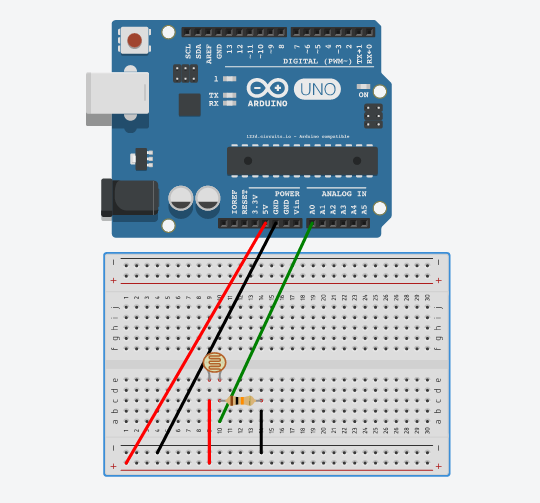
\includegraphics[width=\textwidth]{Design/PhotoSensorTests/Images/photoresistor_setup.png}
  \caption{The figure depicts wiring for a photoresistor with a pulldown resistor.}
  \label{fig:arduino_photoresistor_wiring}
\end{figure}

\subsubsection{Experiments}
In order to find out relevant properties of the two photoresistors, some experiments were conducted. The goals of the experiments are the following:

\begin{itemize}
  \item Determine the precision of the sensor
  \item Find the ideal configuration of resistors in a generic use-case scenario
\end{itemize}

\paragraph{Precision}\label{subsub:precision}
To test the precision of the photoresistors, an experiment was designed.
\subparagraph{Hypothesis}
It was expected that the photoresistors would exhibit some imprecision, as they were cheap, amateur-grade resistors.
\subparagraph{Test Procedure}
To test the precision of the photoresistors, they were put through three different tests. In each test, the resistors were exposed to constant light. Under these constant light conditions, many readings were taken from the resistors, in order to find the variance which they exhibited.
The tests varied in the amount of light exposed to the resistors. The light levels for the tests are the following:

\begin{description}
  \item[Minimal light]
  This scenario was constructed by placing the resistors under a staircase, in a room with only low ambient light from a normal office hallway.
  \item[Average room light]
  This scenario was constructed by placing the resistors in a small, empty room with no windows, with a single light bulb lit.
  \item[Intense light]
  This scenario was constructed by aiming a flashlight directly at the resistors at point blank range.
\end{description}

To record the readings from the resistors, the code in \cref{lst:arduinoPhotoCode} was used for the Arduino. This program simply reads the value from the two sensors and prints it to the serial output, which in this case was a connected computer.

\lstset{language=C}
\begin{lstlisting}[label = lst:arduinoPhotoCode, caption = Arduino program for photoresistor tests]
#define sensor1Pin 0
#define sensor2Pin 1
void setup() {
  Serial.begin(9600);
}

void loop() {
  int val1 = analogRead(sensor1Pin);
  int val2 = analogRead(sensor2Pin);
  Serial.print(val1);
  Serial.print(",");
  Serial.print(val2);
  Serial.print("\n");
}
\end{lstlisting}

This program was run until more than 1000 readings were taken in each scenario.
To find the minimum, maximum and average values, as well as the difference between maximum and minimum in percent.\ranote{Gio asks if we mean the 'relative error'. Dont think that we do, but then what should anything be changed?} The data was copied into a file, which was then input to the C\#-program seen in \cref{lst:cShPhotoCode}.

\lstset{language=[Sharp]C}
\begin{lstlisting}[label = lst:cShPhotoCode, caption = C\# data processing code]
using System;
using System.IO;

namespace ArduinoPhotoTest {
  class Program {
    [STAThreadAttribute]
    static void Main(string[] args) {
      StreamReader file = new StreamReader(@"Path/To/File.txt");
      string line;
      int a0Min = 99999;
      int a1Min = 99999;
      int a0Avg = 0;
      int a1Avg = 0;
      int a0Max = 0;
      int a1Max = 0;
      int counter = 0;
      while ((line = file.ReadLine()) != null) {
        int a0 = Convert.ToInt32(line.Split(',')[0]);
        int a1 = Convert.ToInt32(line.Split(',')[1]);
        a0Avg += a0;
        a1Avg += a1;
        if (a0Min > a0) a0Min = a0;
        else if (a0Max < a0) a0Max = a0;
        if (a1Min > a1) a1Min = a1;
        else if (a1Max < a1) a1Max = a1;
        counter++;
      }
      a0Avg /= counter;
      a1Avg /= counter;
      double a0Diff = ((double)a0Max / (double)a0Min) * 100d - 100;
      double a1Diff = ((double)a1Max / (double)a1Min) * 100d - 100;
      string text = string.Format("a0Avg = {0}\na0Min = {1}
                                  \na0Max = {2}\na0Diff = {6}
                                  %\na1Avg = {3}\na1Min = {4}
                                  \na1Max = {5}\na1Diff = {7}%",
        a0Avg, a0Min, a0Max, a1Avg, a1Min, a1Max, a0Diff, a1Diff);
      Console.WriteLine(text);
      System.Windows.Forms.Clipboard.SetText(text);
      Console.Read();
    }
  }
}
\end{lstlisting}
\subparagraph{Results}
The results of the tests can be seen in \cref{tab:precisionTestResults}. \ranote{does this need to be here. Moved the defination of s1 and s2, down to the table 4.2 caption}

  \begin{table}
\rowcolors{1}{white}{lightgray}
    \centering
    \begin{tabular}[H!]{m{4.5em} c c c c c c c c}
      Scenario & S1 min & S1 max & S1 avg & S1 diff & S2 min & S2 max & S2 avg & S2 diff \\
      \hline
      Minimum light & 136 & 138 & 137 & 1,47 \% & 25 & 27 & 26 & 8.00 \% \\
      Average room light & 875 & 889 & 883 & 1,60 \%  & 634 & 675 & 656 & 6,47 \% \\
      Intense light & 931 & 933 & 932 & 0,21 \%  & 772 & 775 & 773 & 0,39 \% \\
    \end{tabular}
    \caption{Precision test results. "S1" refers to the first photoresistor. and "S2" refers to the second.}\label{tab:precisionTestResults}
  \end{table}
\ranote{look at colloum headers, combine them?}
\subparagraph{Partial Conclusion}
As expected, the resistors did exhibit some imprecision under constant light. S2, however, was much worse than S1 under the minimum and average light scenarios, having more than 5 times the difference between minimum and maximum values. Both S1 and S2 were very consistent under intense light. \ranote{Not enough analysis, simply reading the result is pointless. Delete tha sub-paragraph? Or what did we wanna say?}

\paragraph{Configuration}
In order fully take advantage of the two photoresistors, an experiment was devised to find a configuration of pull-down resistors, which would offer a large range of meaningful values, i.e. be able to detect small differences under low light as well as intense light scenarios.
\subparagraph{Hypothesis}
Using different pull-down resistors on the photoresistors would make it possible to extend the range of values, which the sensor pair could register.
\subparagraph{Test Procedure}
The scenarios described in \cref{subsub:precision} are also used in this experiment. Between each set of scenarios, a pull-down resistor value was changed.\ranote{Gio doesn't understand, if changes in photoresistor intro works should solve this as well.} As the 10K $\Omega$ resistor used in the previous experiments responded well to low light conditions, and was almost impossible to bottom out, another resistor-value was sought which could complement this. To increase the tolerance to light, available resistors with less resistance than 10K $\Omega$ have been investigated.
\subparagraph{Results}
The results from the configuration experiments can be seen in \cref{tab:1KTestResults,tab:2.2KTestResults,tab:4.4KTestResults,tab:10KTestResults,tab:12.2KTestResults}.

\begin{table}[H]
\rowcolors{1}{white}{lightgray}
  \centering
  \begin{tabular}{l c c c c}
    Scenario & 1K $\Omega$ min & 1K $\Omega$ max & 1K $\Omega$ avg & 1K $\Omega$ diff \\
    \hline
    Minimum light & 0 & 0 & 0 & 0.00 \% \\
    Average room light & 16 & 18 & 17 & 12.50 \% \\
    Intense light & 406 & 408 & 406 & 0.49 \% \\
  \end{tabular}
  \caption{1K $\Omega$ resistor results}\label{tab:1KTestResults}
\end{table}

\begin{table}[H]
\rowcolors{1}{white}{lightgray}
  \centering
  \begin{tabular}{l c c c c}
    Scenario & 1K $\Omega$ min & 2.2K $\Omega$ max & 2.2K $\Omega$ avg & 2.2K $\Omega$ diff \\
    \hline
    Minimum light & 0 & 0 & 0 & 0.00 \% \\
    Average room light & 49 & 58 & 53 & 18.37 \% \\
    Intense light & 609 & 612 & 610 & 0.49 \% \\
  \end{tabular}
  \caption{2.2K $\Omega$ resistor results}\label{tab:2.2KTestResults}
\end{table}

\begin{table}[H]
\rowcolors{1}{white}{lightgray}
  \centering
  \begin{tabular}{l c c c c}
    Scenario & 4.4K $\Omega$ min & 4.4K $\Omega$ max & 4.4K $\Omega$ avg & 4.4K $\Omega$ diff \\
    \hline
    Minimum light & 7 & 11 & 11 & 57.14 \% \\
    Average room light & 282 & 287 & 284 & 1.77 \% \\
    Intense light & 893 & 895 & 894 & 0.22 \% \\
  \end{tabular}
  \caption{4.4K $\Omega$ resistor results}\label{tab:4.4KTestResults}
\end{table}

\begin{table}[H]
\rowcolors{1}{white}{lightgray}
  \centering
  \begin{tabular}{l c c c c}
    Scenario & 10K $\Omega$ min & 10K $\Omega$ max & 10K $\Omega$ avg & 10K $\Omega$ diff \\
    \hline
    Minimum light & 136 & 138 & 137 & 1.47 \% \\
    Average room light & 875 & 889 & 883 & 1.60 \% \\
    Intense light & 931 & 933 & 932 & 0.21 \% \\
  \end{tabular}
  \caption {10K $\Omega$ resistor results}\label{tab:10KTestResults}
\end{table}

\begin{table}[H]
  \rowcolors{1}{white}{lightgray}
  \centering
  \begin{tabular}{l c c c c}
    Scenario & 12.2K $\Omega$ min & 12.2K $\Omega$ max & 12.2K $\Omega$ avg & 12.2K $\Omega$ diff \\
    \hline
    Minimum light & 44 & 52 & 51 & 18.18 \% \\
    Average room light & 592 & 622 & 606 & 5.07 \% \\
    Intense light & 979 & 982 & 980 & 0.31 \% \\
  \end{tabular}
  \caption{12.2K $\Omega$ resistor results}\label{tab:12.2KTestResults}
\end{table}

\subparagraph{Partial Conclusion}
Using a 12.2K pull-down resistor on one photoresistor and a 4.4K pull-down resistor on the other allows for good precision both in darker and lighter envoirments, because one photoresistor is very sensitive to low light conditions and very tolerant\ranote{intolerant?} of intense light conditions, and the other is the inverse. This pairing seems more than adequate for the purpose in this project.

